% =====================================================================
% SCAFFOLD ONLY --- pending analysis/run_all.py
% No results exist yet. This section fixes the table and figure schedule,
% their labels, captions and the \gen* macros each will consume, so that
% analysis/emit_tex_values.py can be written against a settled contract.
% Every numeric claim below is a \gen* macro; missing keys emit \GENMISSING
% so a stale results/ tree fails visibly at build time. Prose around the
% macros is written in final form where the sign or ordering of the result
% is implied by construction, and left deliberately neutral where it is not.
% =====================================================================

\section{Results}
\label{sec:results}

I report the price path first, then first-order incidence by decile, then the constituency crossing that is the paper's central object, then the policy scorecard. Unless stated otherwise, figures are for the realised 2026 scenario; the baseline and adverse scenarios bound it and are reported alongside. All losses are annual, in 2026 prices, and expressed both in pounds and as a share of equivalised disposable income on the HBAI concept.

\subsection{The price path}
\label{sec:results-prices}

Table~\ref{tab:pricepath} reports the modelled quarterly path of the Ofgem default tariff cap and of pump prices under each scenario, alongside the wholesale inputs that generate them through equation~\eqref{eq:passthrough}. Under the realised scenario the annualised gas unit rate rises \genGasUnitRatePct{} per cent and the electricity unit rate \genElecUnitRatePct{} per cent, the asymmetry reflecting the smaller wholesale share of the electricity cap; the annualised dual-fuel cap for a typical household reaches \pounds \genCapAnnualised{} against \pounds \genCapBaselineLevel{} in the pre-shock baseline.

\begin{table}[htbp]
\centering
\caption{Modelled wholesale inputs, Ofgem cap path and pump prices by quarter and scenario. Wholesale columns are forward-window averages; cap columns apply the pass-through coefficient $\phi_f$ and lag $\ell$ of Section~\ref{sec:step1}; the final row annualises by consumption-weighted averaging over the modelled year.}
\label{tab:pricepath}
\begin{tabular}{lrrrrrr}
\toprule
& \multicolumn{2}{c}{Baseline} & \multicolumn{2}{c}{Realised} & \multicolumn{2}{c}{Adverse} \\
\cmidrule(lr){2-3}\cmidrule(lr){4-5}\cmidrule(lr){6-7}
Quarter & Gas & Elec. & Gas & Elec. & Gas & Elec. \\
\midrule
% populated by analysis/emit_tex_values.py from results/price_path.csv
\multicolumn{7}{c}{\emph{[table body generated]}} \\
\bottomrule
\end{tabular}
\end{table}

\begin{figure}[htbp]
\centering
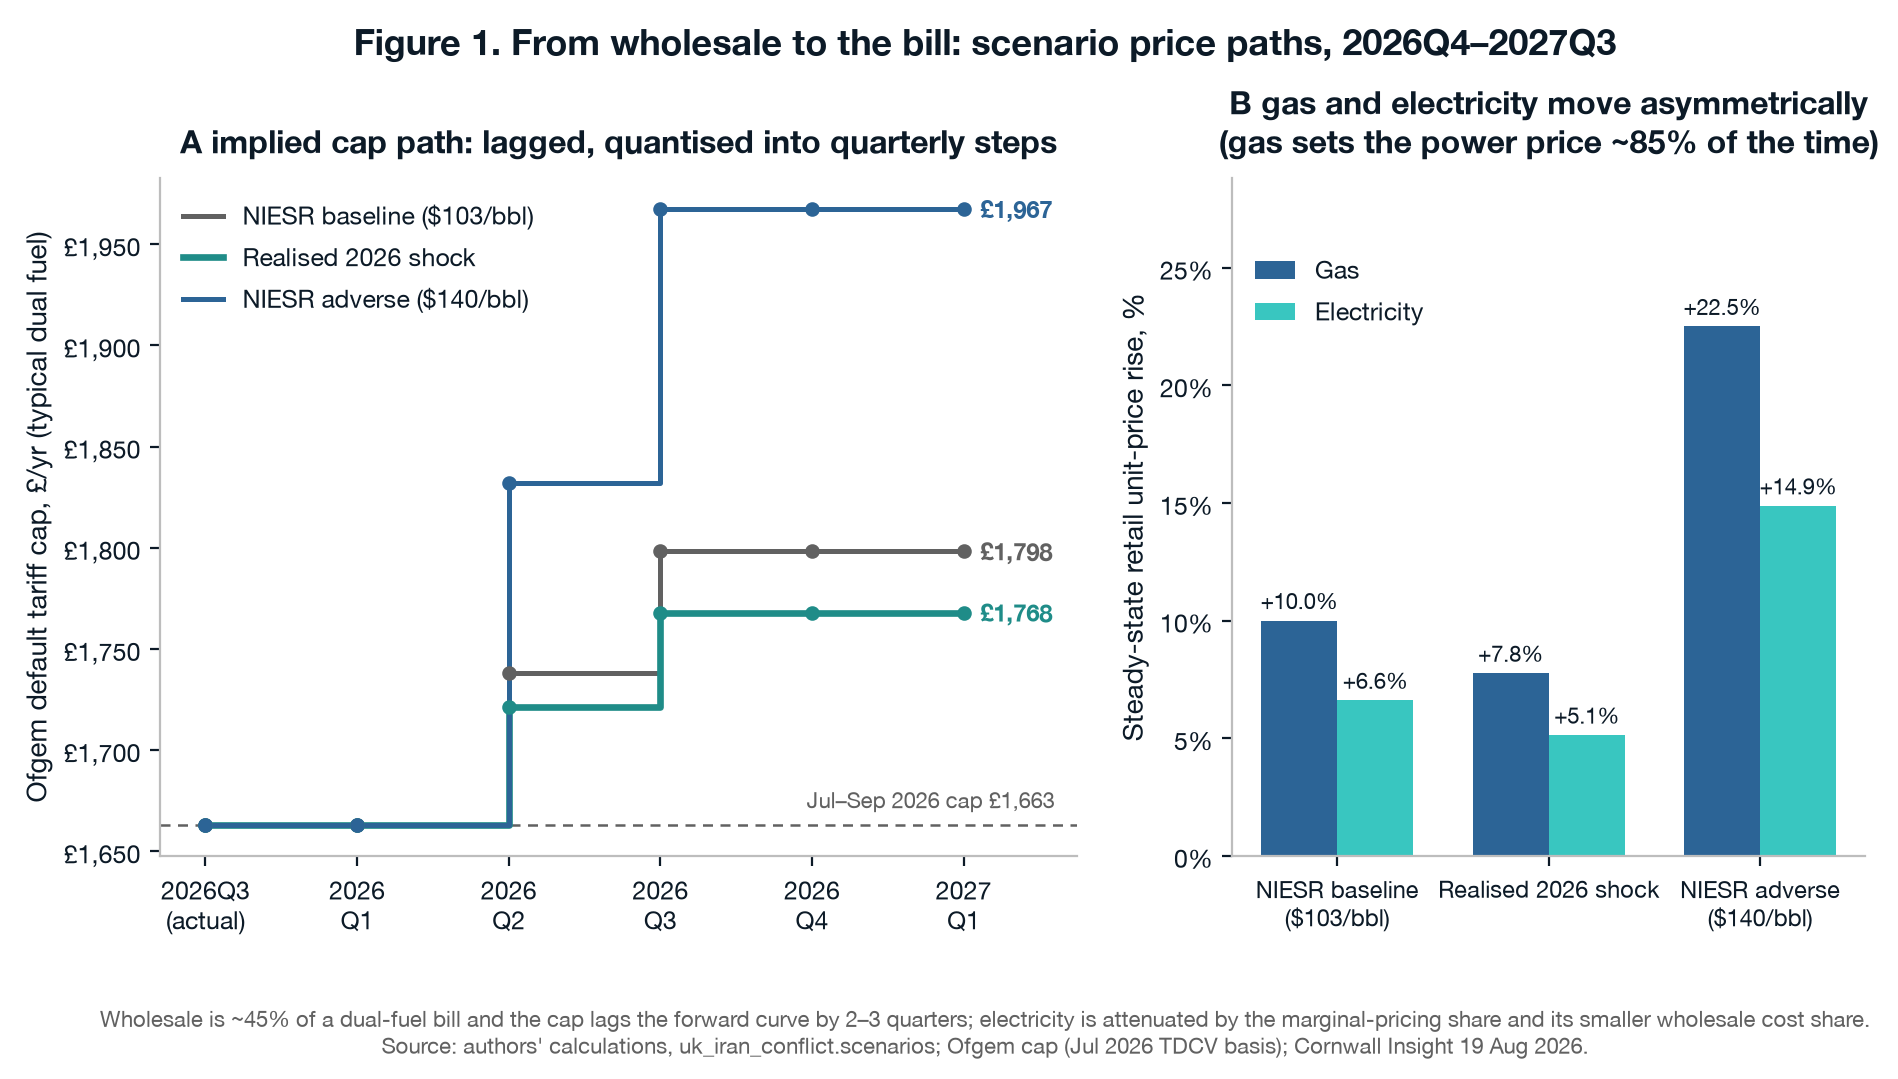
\includegraphics[width=.85\textwidth]{../results/figures/fig1_price_path.png}
\caption{Wholesale gas and oil paths and the implied Ofgem cap and pump-price paths, by scenario. The visible horizontal displacement between the wholesale series and the cap series is the two-to-three-quarter averaging lag; the vertical compression is the wholesale share of the bill.}
\label{fig:pricepath}
\end{figure}

Figure~\ref{fig:pricepath} makes the two transmission features visible at once: the lag between the wholesale move and the household bill, and the attenuation from the non-commodity components of the cap. It is also the figure that shows why peak-based bill-rise estimates in the policy literature exceed annualised ones.

\subsection{First-order incidence by decile}
\label{sec:results-decile}

Table~\ref{tab:decile} reports the annual cost increase by equivalised disposable income decile in pounds and as a share of income. The mean household loses \pounds \genCentralLossMean{}, or \genCentralLossPctIncome{} per cent of income. The two orderings diverge by construction of the underlying data rather than by assumption: in cash the loss rises across deciles, from \pounds \genDecileOneLossGbp{} in decile one to \pounds \genDecileTenLossGbp{} in decile ten, while as a share of income it falls, from \genDecileOneLossPct{} per cent to \genDecileTenLossPct{} per cent. The ratio of the bottom-decile to top-decile percentage loss is \genDecileRatioPct{}.

\begin{table}[htbp]
\centering
\caption{Annual household energy cost increase by equivalised disposable income decile, realised scenario: mean pound loss, loss as a share of equivalised disposable income, and the decomposition into gas, electricity and road fuel. Gross of any policy response.}
\label{tab:decile}
\begin{tabular}{lrrrrr}
\toprule
Decile & \pounds\ loss & \% of income & Gas & Electricity & Road fuel \\
\midrule
% populated from results/decile_incidence.csv
\multicolumn{6}{c}{\emph{[table body generated]}} \\
\bottomrule
\end{tabular}
\end{table}

\begin{figure}[htbp]
\centering
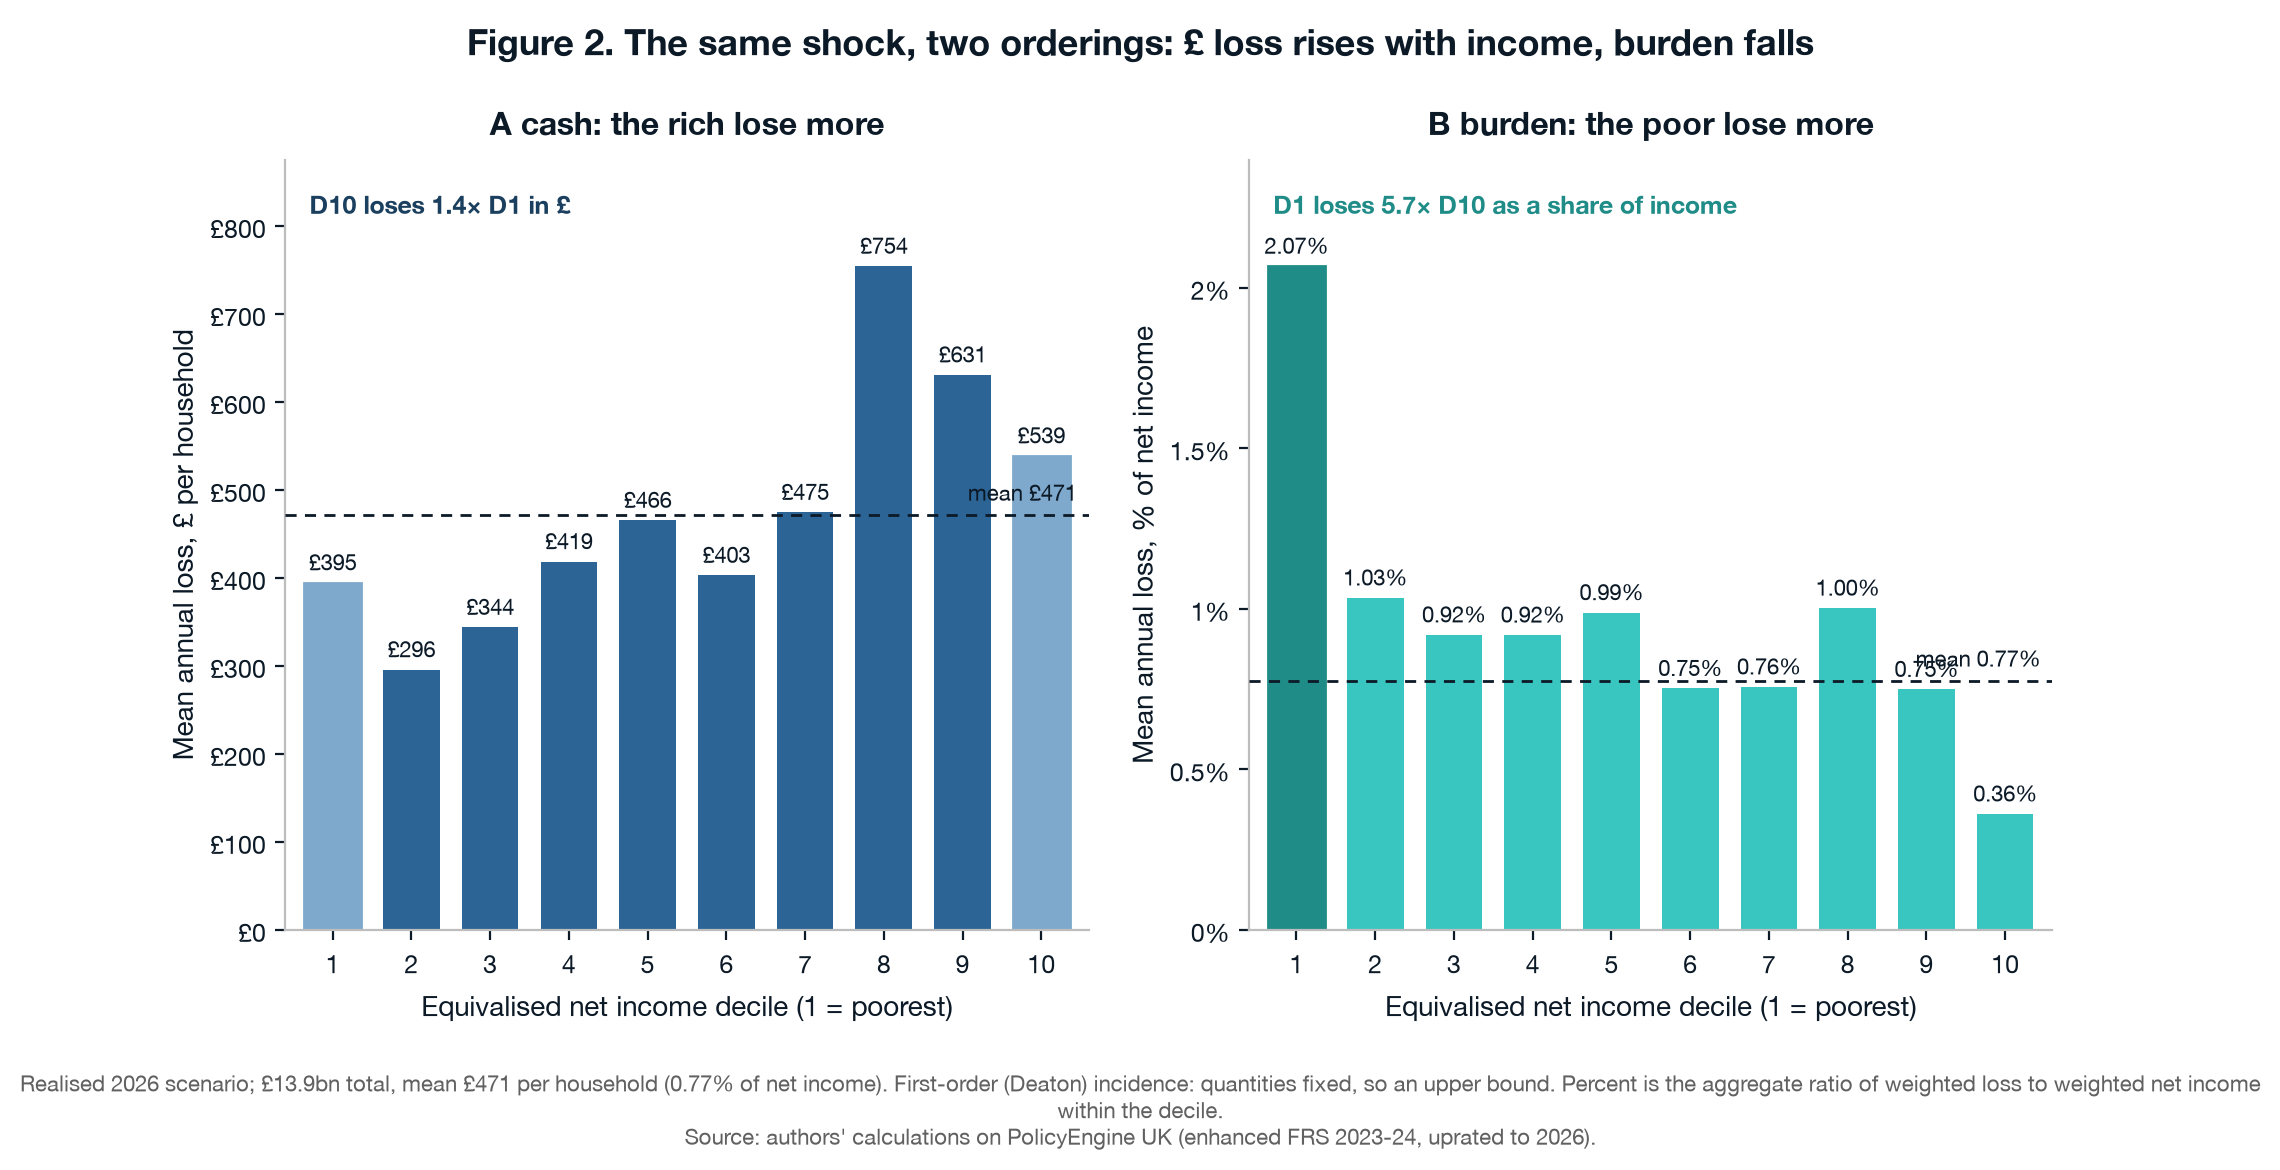
\includegraphics[width=.85\textwidth]{../results/figures/fig2_decile_dual.png}
\caption{Energy cost increase by income decile on two metrics: bars give the mean loss in pounds (left axis), the line gives the loss as a share of equivalised disposable income (right axis). The crossing of the two series is the paper's organising fact.}
\label{fig:deciledual}
\end{figure}

\begin{figure}[htbp]
\centering
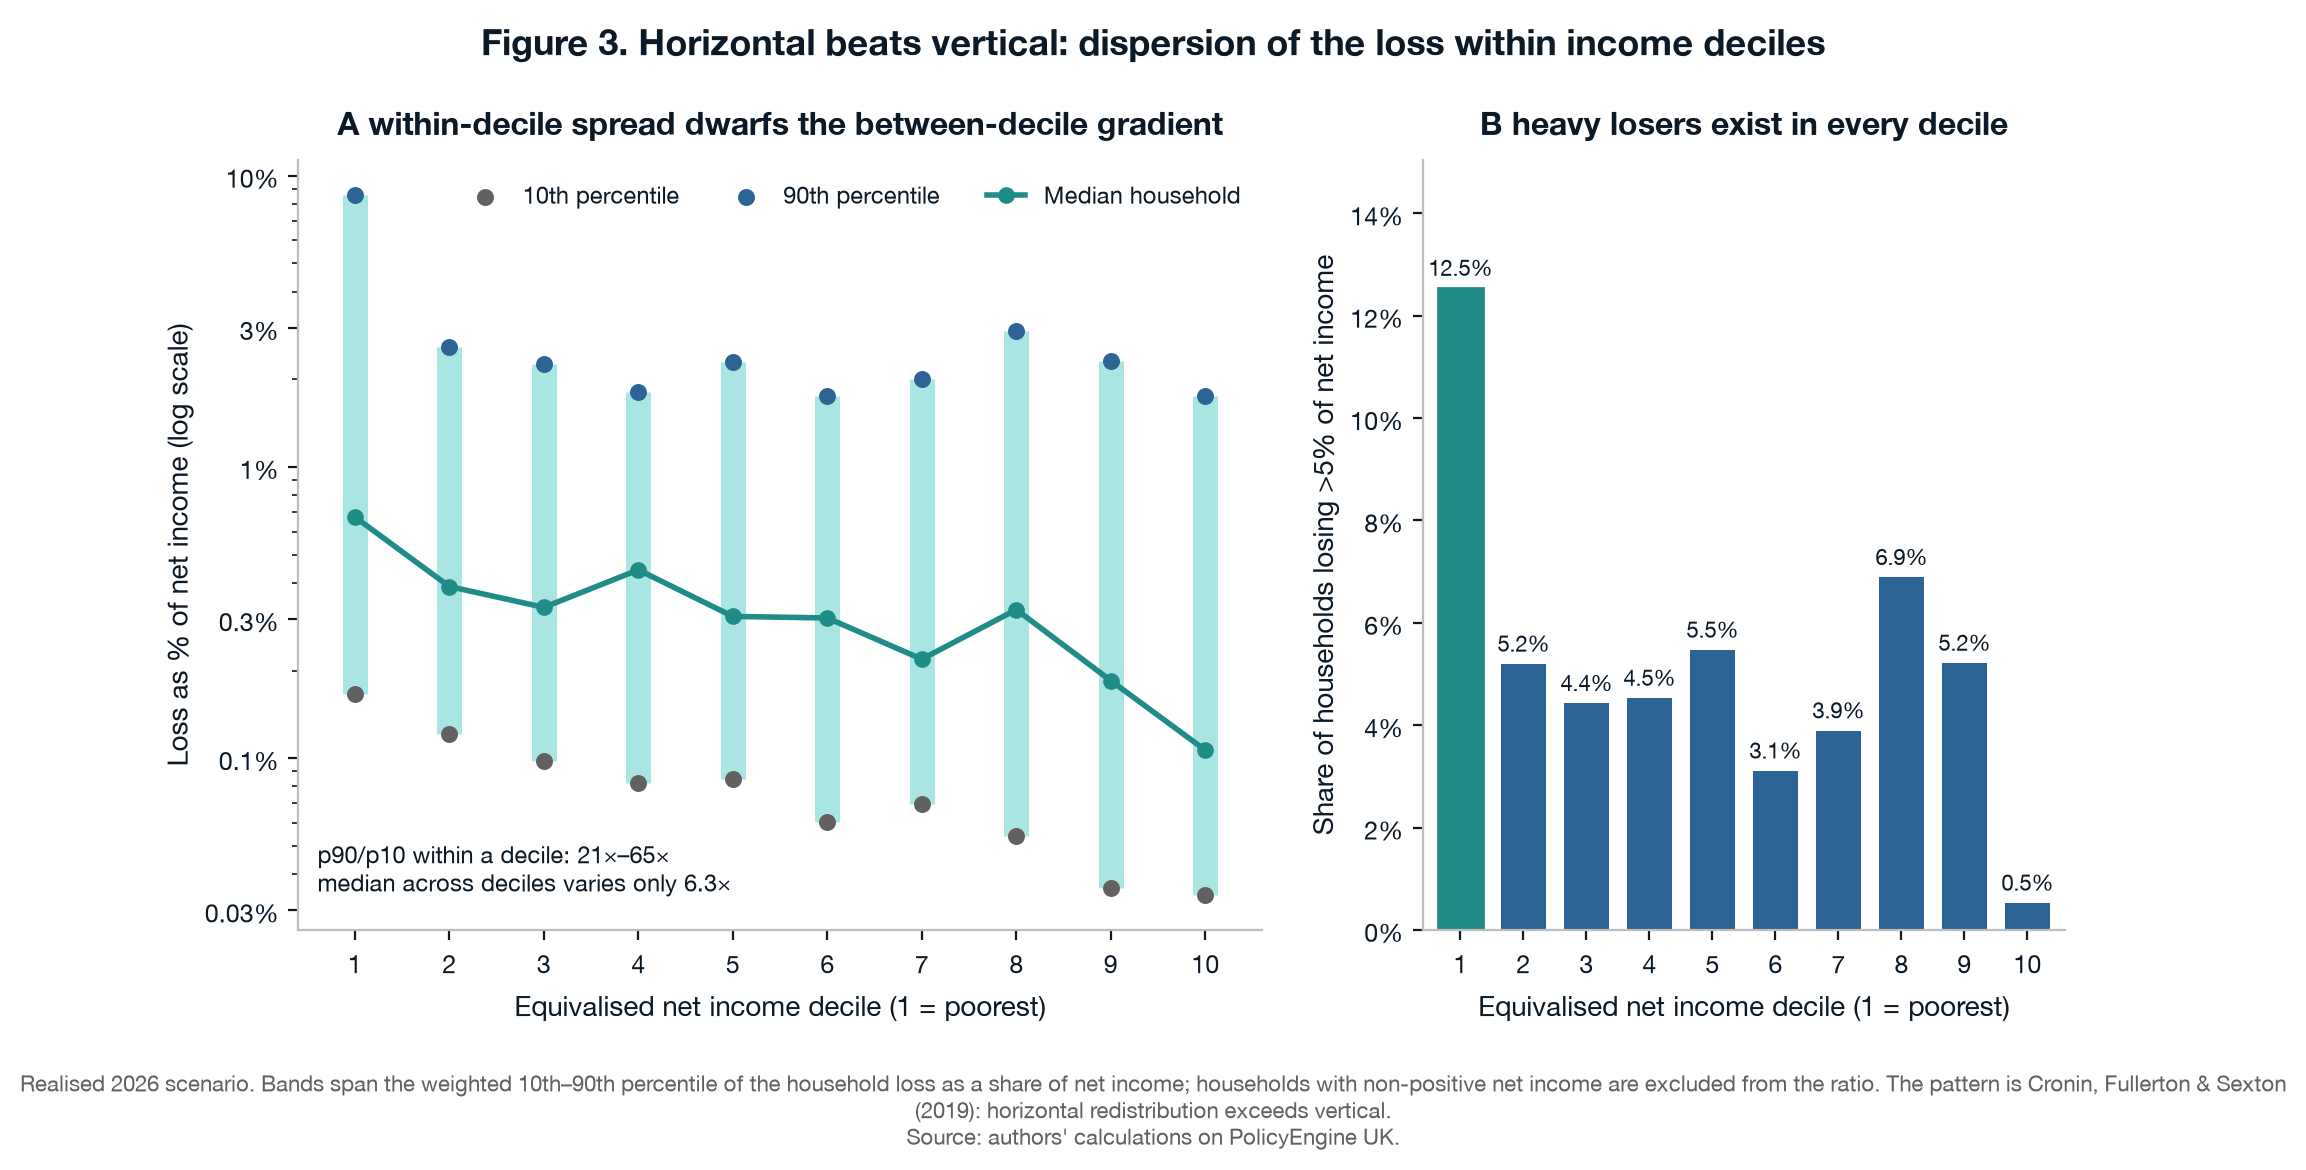
\includegraphics[width=.85\textwidth]{../results/figures/fig3_within_decile.png}
\caption{Within-decile dispersion of the percentage loss: box plots by decile with whiskers at the 10th and 90th percentiles. Shows how far horizontal dispersion inside each decile exceeds the vertical gradient across deciles.}
\label{fig:withindecile}
\end{figure}

Figure~\ref{fig:withindecile} is the within-decile counterpart. The interdecile range of the mean percentage loss is \genBetweenDecileRangePct{} percentage points, while the mean within-decile interdecile range is \genWithinDecileRangePct{} percentage points --- the quantitative form of the \citet{cronin2019} point, and the reason the uncompensated-loser metric in Section~\ref{sec:results-policy} does work that decile averages cannot.

\subsection{Fuel-mix and heating-type heterogeneity}
\label{sec:results-heterogeneity}

Table~\ref{tab:heating} breaks losses down by primary heating fuel and by on- versus off-gas-grid status. Because the shock is applied asymmetrically to gas and electricity, the ranking of household types is a direct consequence of the Step 1 calibration and not of the microdata alone: gas-heated households absorb the larger unit-rate move, while electrically heated and off-grid households face a smaller proportional move from a higher baseline unit cost. Off-gas-grid households lose \pounds \genOffGridLossGbp{} on average against \pounds \genOnGridLossGbp{} on grid.

\begin{table}[htbp]
\centering
\caption{Losses by primary heating fuel, gas-grid connection, tenure and household composition, realised scenario. Reported in pounds and as a share of income, with the population share of each group.}
\label{tab:heating}
\begin{tabular}{lrrr}
\toprule
Group & Population share & \pounds\ loss & \% of income \\
\midrule
% populated from results/heterogeneity.csv
\multicolumn{4}{c}{\emph{[table body generated]}} \\
\bottomrule
\end{tabular}
\end{table}

\subsection{Incidence by parliamentary constituency}
\label{sec:results-constituency}

Figure~\ref{fig:maps} is the paper's headline result: the same shock mapped across all 650 Westminster constituencies on the two metrics side by side. The left panel shades each seat by mean loss as a share of income; the right panel shades the same seats by mean loss in pounds. The two maps are close to negatives of one another. The Spearman rank correlation between the two constituency rankings is \genConstituencyRankCorr{}, and of the fifty seats worst affected in percentage terms only \genTailOverlapCount{} also appear among the fifty worst affected in pounds.

\begin{figure}[htbp]
\centering
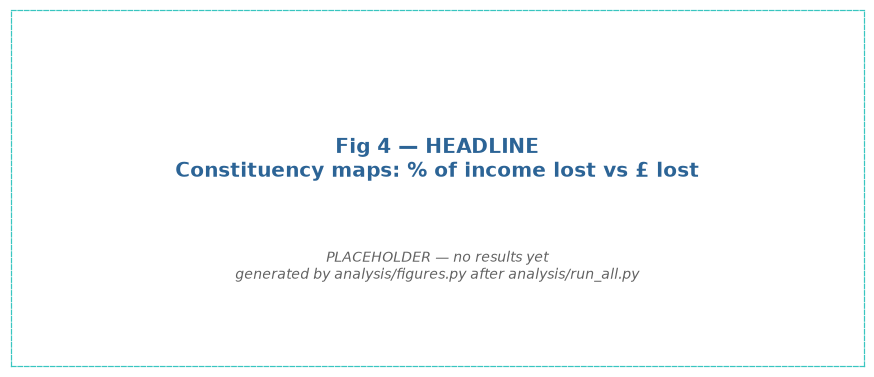
\includegraphics[width=\textwidth]{../results/figures/fig4_constituency_maps.png}
\caption{Energy cost increase by Westminster parliamentary constituency, realised scenario. Left: mean loss as a share of equivalised disposable income. Right: mean loss in pounds per year. Same shock, same households, same colour scale quantiles --- opposite geographies. Constituency estimates rest on re-optimised synthetic weights (Section~\ref{sec:limitations}); rankings are more reliable than levels.}
\label{fig:maps}
\end{figure}

\begin{figure}[htbp]
\centering
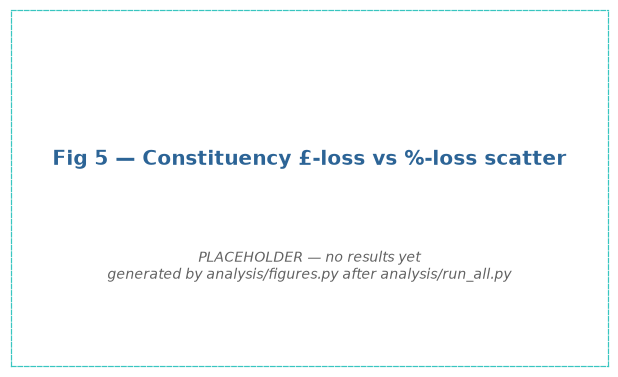
\includegraphics[width=.75\textwidth]{../results/figures/fig5_constituency_scatter.png}
\caption{Constituency-level scatter of pound loss against percentage-of-income loss, with seats in either tail labelled and marker size proportional to the seat's share of households on means-tested benefits. The scatter quantifies what the paired maps show qualitatively.}
\label{fig:constituencyscatter}
\end{figure}

\begin{table}[htbp]
\centering
\caption{The twenty constituencies worst affected on each metric, side by side, with each seat's rank on the other metric. Illustrates directly that a policy calibrated to one ranking misses the other.}
\label{tab:worstseats}
\begin{tabular}{lrrlrr}
\toprule
\multicolumn{3}{c}{Worst by \% of income} & \multicolumn{3}{c}{Worst by \pounds} \\
\cmidrule(lr){1-3}\cmidrule(lr){4-6}
Constituency & \% & \pounds\ rank & Constituency & \pounds & \% rank \\
\midrule
% populated from results/constituency_incidence.csv
\multicolumn{6}{c}{\emph{[table body generated]}} \\
\bottomrule
\end{tabular}
\end{table}

\subsection{Scenario comparison}
\label{sec:results-scenario}

Table~\ref{tab:scenario} sets the three scenarios against one another on the headline aggregates: total additional household energy spending, the mean loss, the bottom-decile percentage loss, and the number of households pushed below the fuel-poverty and relative-poverty thresholds. Aggregate additional household energy and fuel spending is \pounds \genAggSpendRealisedBn{} billion in the realised scenario against \pounds \genAggSpendAdverseBn{} billion in the adverse one.

\begin{table}[htbp]
\centering
\caption{Headline aggregates under the baseline, realised and adverse scenarios. Static, use-side only, zero-elasticity; see Section~\ref{sec:limitations}.}
\label{tab:scenario}
\begin{tabular}{lrrr}
\toprule
& Baseline & Realised & Adverse \\
\midrule
% populated from results/scenario_summary.csv
\multicolumn{4}{c}{\emph{[table body generated]}} \\
\bottomrule
\end{tabular}
\end{table}

\subsection{Scoring the policy responses}
\label{sec:results-policy}

Table~\ref{tab:scorecard} scores the five responses of Section~\ref{sec:step4} on the three metrics. The means-tested social tariff delivers \genSocialTariffShareBottomThree{} per cent of its spend to deciles one to three at a cost of \pounds \genSocialTariffCostBn{} billion, but leaves \genSocialTariffUncompensatedShare{} per cent of losing households uncompensated. The JRF universal discounted block costs \pounds \genJrfCostBn{} billion and leaves \genJrfUncompensatedShare{} per cent uncompensated, delivering \genJrfShareBottomThree{} per cent of spend to deciles one to three. The Warm Home Discount expansion costs \pounds \genWhdCostBn{} billion; the VAT cut on domestic fuel costs \pounds \genVatCutCostBn{} billion and delivers \genVatCutShareBottomThree{} per cent to the bottom three deciles; the flat rebate costs \pounds \genRebateCostBn{} billion. Cost per pound of bottom-decile gain runs from \pounds \genBestCostPerPound{} to \pounds \genWorstCostPerPound{} across the five.

\begin{table}[htbp]
\centering
\caption{Policy scorecard: exchequer cost, cost per pound of bottom-decile gain, share of spend reaching deciles one to three, and share of losing households left uncompensated, for each of the five responses, evaluated against the realised scenario.}
\label{tab:scorecard}
\begin{tabular}{lrrrr}
\toprule
Reform & Cost (\pounds bn) & \pounds\ per \pounds\ D1 gain & \% to D1--D3 & \% losers uncompensated \\
\midrule
% populated from results/policy_scorecard.csv
\multicolumn{5}{c}{\emph{[table body generated]}} \\
\bottomrule
\end{tabular}
\end{table}

\begin{figure}[htbp]
\centering
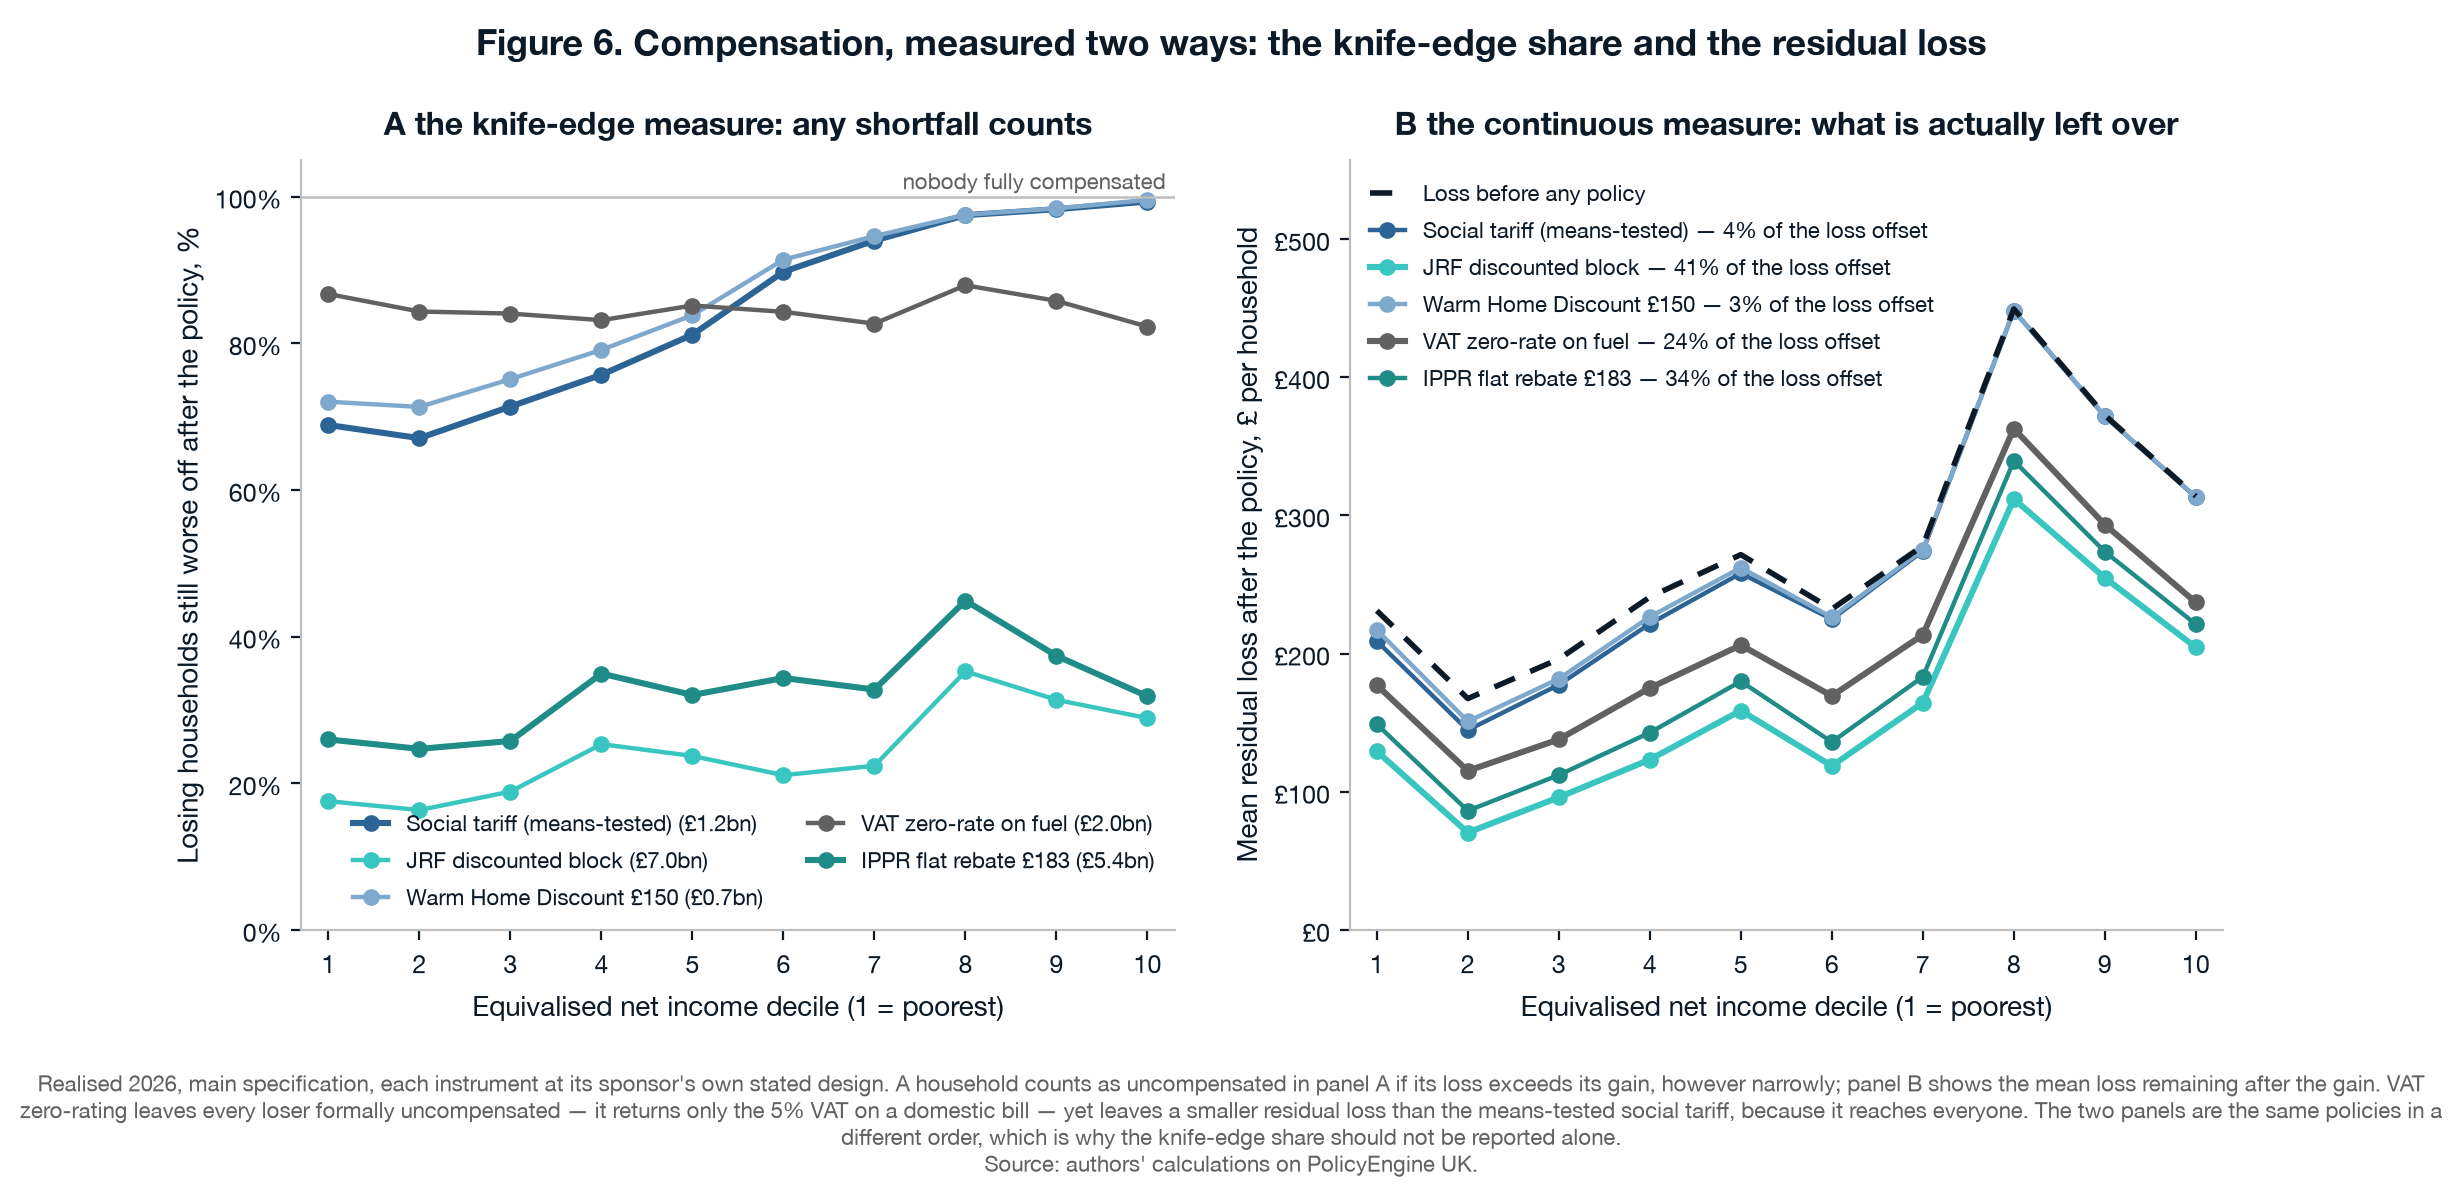
\includegraphics[width=\textwidth]{../results/figures/fig6_uncompensated.png}
\caption{Share of losing households left uncompensated within each income decile, by policy. The between-decile targeting metrics rank the policies one way; this within-decile metric ranks them differently, which is the substance of Section~\ref{sec:policy}.}
\label{fig:uncompensated}
\end{figure}

\begin{figure}[htbp]
\centering
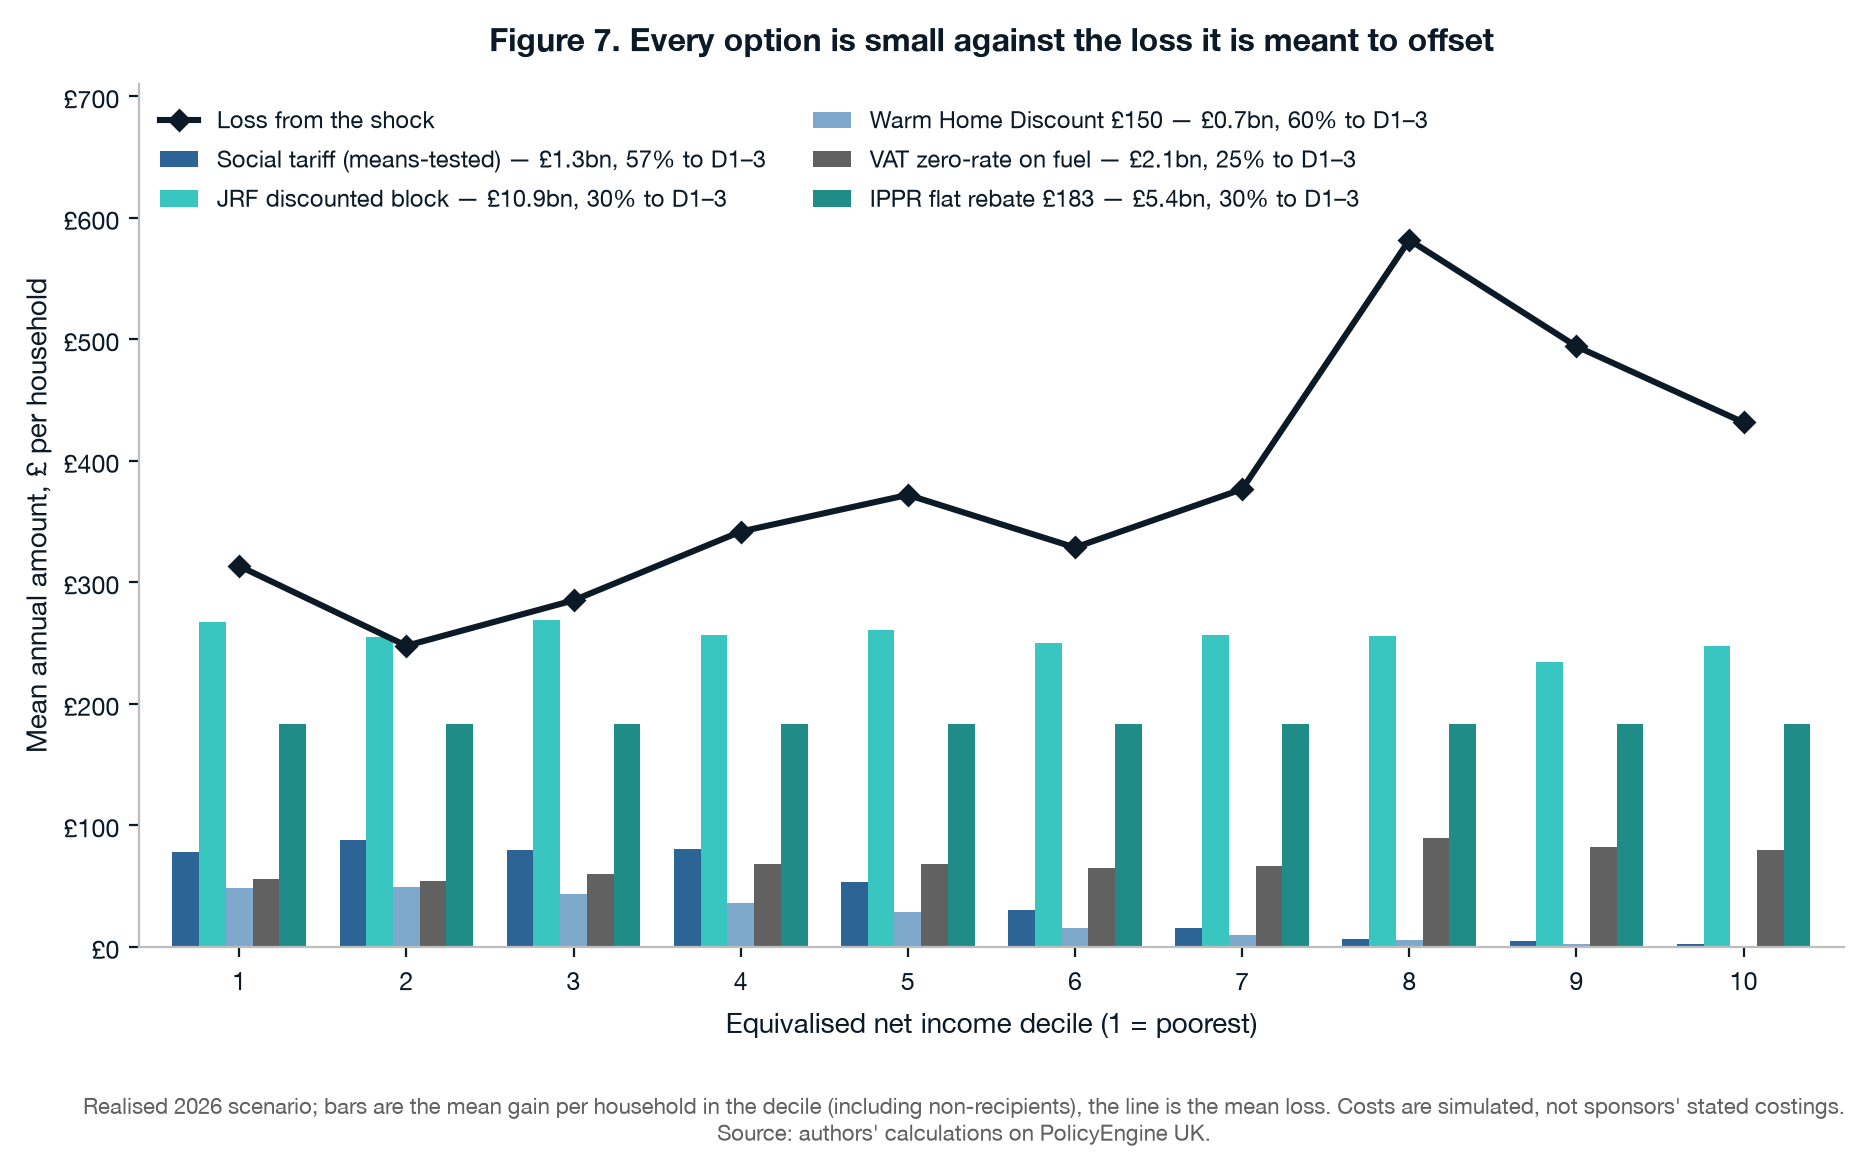
\includegraphics[width=.85\textwidth]{../results/figures/fig7_policy_deciles.png}
\caption{Net change in household disposable income by decile under each policy, shock included, as a share of baseline income. Shows which policies fully offset the shock at the bottom and where each leaves a residual loss.}
\label{fig:policydeciles}
\end{figure}

\begin{figure}[htbp]
\centering
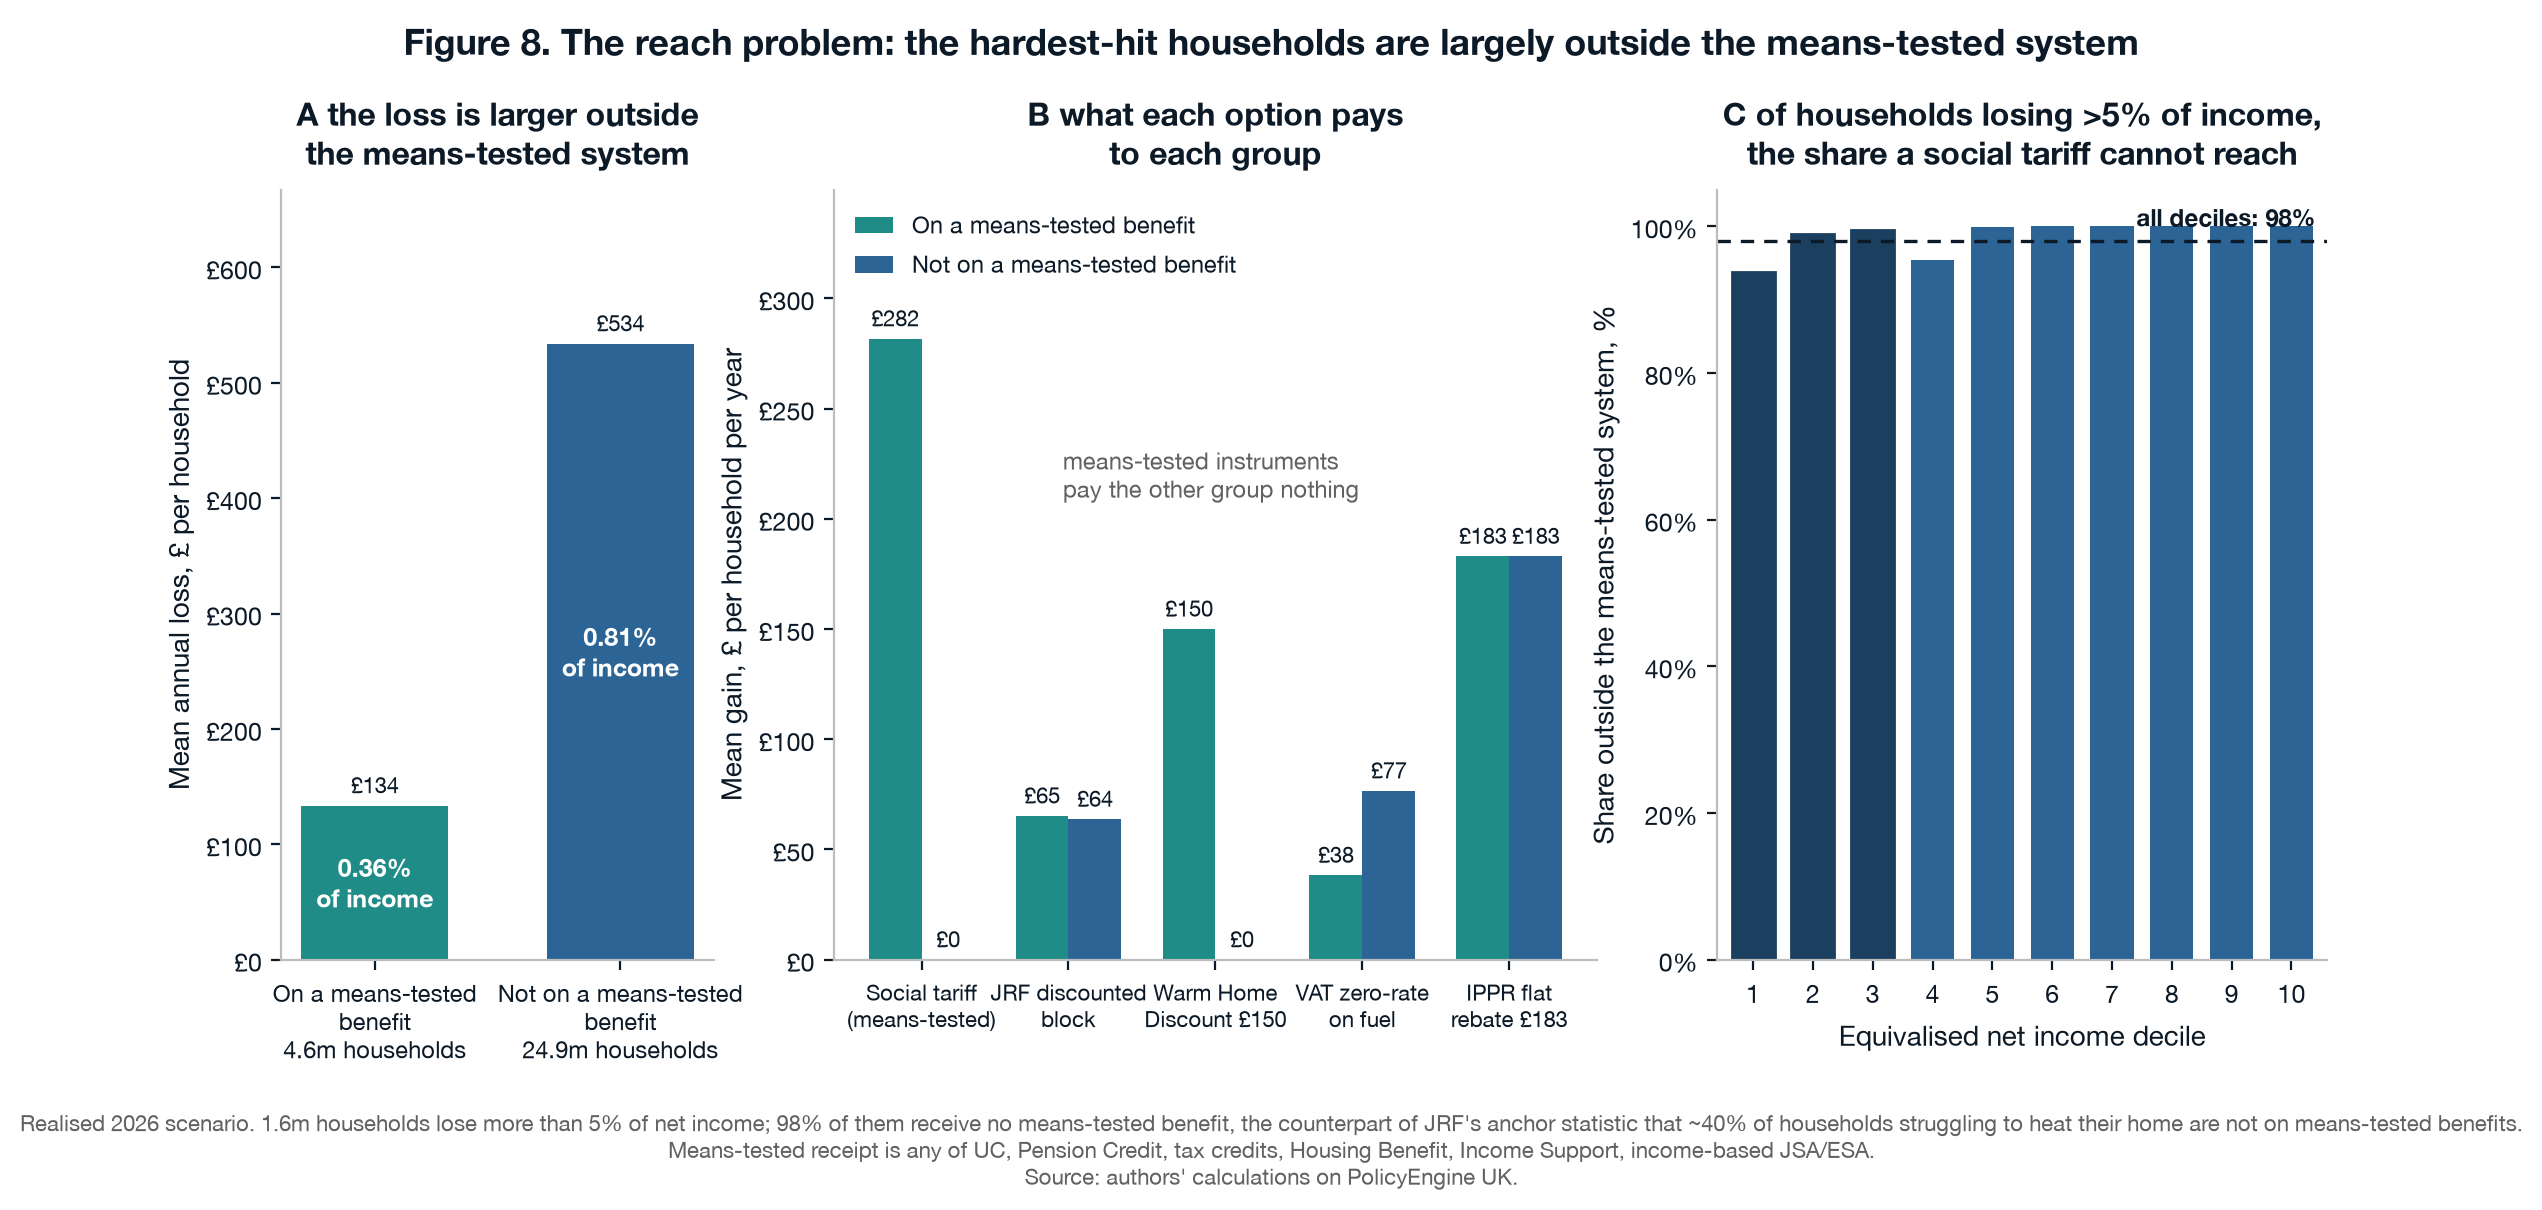
\includegraphics[width=.85\textwidth]{../results/figures/fig8_benefit_status.png}
\caption{Compensation rates split by receipt of means-tested benefits. The quantitative form of the \genNonMeansTestedStruggling{} per cent statistic: the share of struggling households outside the means-tested system, and what each policy delivers to them.}
\label{fig:benefitstatus}
\end{figure}
